\begin{figure*}[h]
\caption{Weekly Mentor Check-Ins For the Six Weeks of the Program, Average Scores}
\label{fig:checkins}
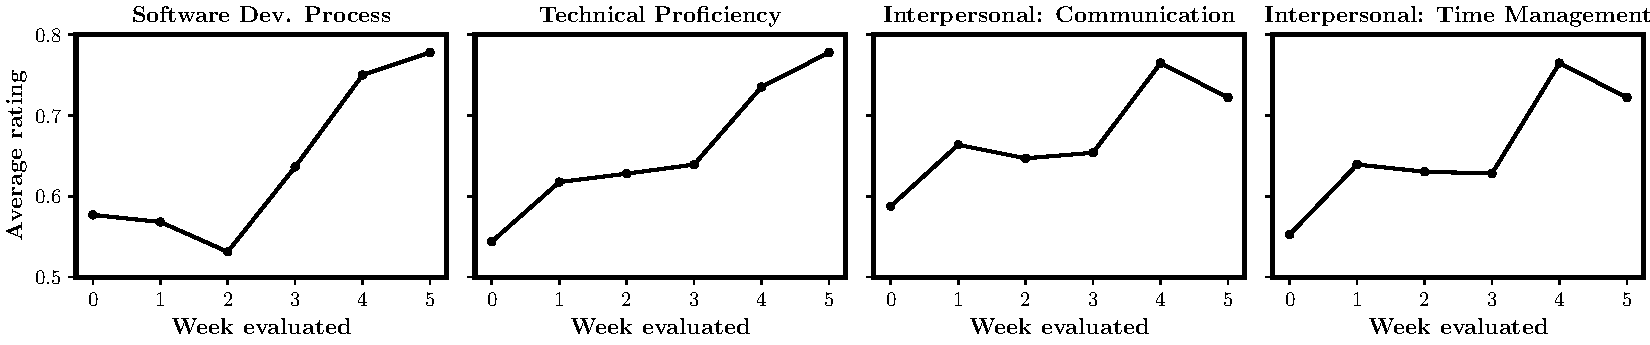
\includegraphics[width=\textwidth]{images/fig-checkins.pdf}
\end{figure*}

\section{Results and Evaluation}

We operated the program in the summers of 2020 and 2021. Except as noted previously, the program was substantially the same in both years. In total 311 students were admitted (197 in 2020 and 114 in 2021).\footnote{The full program also included a "beginner track" to which an additional 145 students were admitted. This track was for high school students who had only completed AP CS A, mentored by college students rather than industry professionals, and students in this track would not qualify for traditional internships. All data from the beginner track is omitted in the results.} All but 5 students completed the program.

80\% of students were undergraduates; specifically: 29\% seniors, 33\% juniors, 27\% sophomores, and 10\% freshmen. 97\% of students had never completed an internship before.

Only 19\% of undergraduates who participated attended an R1 university (which are the schools most commonly targeted by recruiters from technology companies). 30\% attended a non-R1 Doctorate-/Masters granting university, 43\% a Baccalaureate granting college, and 8\% an Associates granting college.

67\% of students were under-represented in technology (51\% were women or non-binary, and 31\% were Black, Latinx, or Native American). Although the program was conducted virtually, 90\% of students were located in the United States.

We matched these students with 125 mentors. Although mentors were volunteers who did not represent their employers, we collected each mentor's employment history. The most popular employer was Microsoft, which accounted for 10\% of mentors. 63\% worked for a Fortune 500 company at the time of mentoring. Mentors had a median of 3 years of full-time work experience. 62\% of mentors had a job title corresponding to Software Engineer, 20\% had a title corresponding to Senior Software Engineer, and 9\% had the title corresponding to Engineering Manager. The most senior mentor was a VP of Engineering for a 200-person technology company.

To evaluate the success of the program, we considered long-term job outcomes, mentor evaluations, and student self-evaluations.


\subsection{Job Placement Outcomes}

Ultimately, we hope internships will lead to employment, and measuring the rate of students who obtained employment was our primary evaluation criteria. Because no one source of data is perfect, to determine employment status we combined information from student follow-up surveys, school reporting data, and public information from LinkedIn and Github.

The NCES reports that one year after graduation, an average of 61.9\% of students with a bachelor's degree in Computer Science secure employment in their field. \cite{DigestEducationStatistics2021} We found that at least 69\% of the graduating seniors who participated in the 2020 program\footnote{We are not able to present longitudinal data for 2021's program due to the timeline of publication.} had secured a full-time job in technology within nine months of the end of the program. This number may be artificially deflated by a lack of available data and suppressed new-grad hiring as a result of the COVID-19 pandemic.

Additionally, we found that at least 60\% of rising seniors had secured a traditional internship within nine months.



\subsection{Mentor Skill Evaluations}

A primary aim of the program was to prepare students for industry work. We asked mentors to evaluate how close each of their mentees was to meeting expectations for a new-grad hire, considering: their ability to work independently through the software development process, their interpersonal skills, and their technical proficiency. (We did not have mentors evaluate cross-functional competencies as these were a part of the larger program.) Mentors could choose "yes, the student already meets new-grad expectations", "on-track to meet by graduation", or "no, needs work". Mentors were asked to assess student skill at the end of each week, as well as provide a final evaluation.

Weekly results were converted to a numeric score (yes = 1, by graduation = 0.5, no = 0) and an average was graphed over time. (Figure \ref{fig:checkins}) Over the course of the program, mentors' ratings of their students improved across all categories by at least 30-40\%. Most notably, student competency in the software development process improved by 60\% between weeks 2-4. (This corresponds to student remarks from the first two weeks that they were struggling to succeed without the direct guidance they were used to from school.)

The final results, presented in Table \ref{tab:mentors}, paint a positive picture, with mentors indicating that over half of students already meet their expectations and they expect 90\% to do so by the time they graduate.

Mentors also indicated they would be willing to provide a positive employment reference for 82\% of students who participated in the program. (That number increased to 95\% for students who were rated as "on-track to meet by graduation" or higher in all four evaluation criteria.)

\begin{table}[]
\caption{Mentor Final Evaluation of Student Skills}
\label{tab:mentors}
\begin{tabular}{llccc}
 && \textbf{Yes} & \textbf{By Graduation} & \textbf{No} \\
\multicolumn{2}{@{}l}{Software Development Process} & 56\% & 37\% & 7\% \\
\multicolumn{5}{@{}l}{Interpersonal} \\
&Communication & 56\% & 40\% & 4\% \\
&Time Management & 55\% & 40\% & 5\% \\
\multicolumn{2}{@{}l}{Technical Proficiency} & 41\% & 53\% & 6\% \\
\end{tabular}
\end{table}

Overall, mentors said agreed with the decision to admit their mentees 91\% of the time, but only thought 64\% of students were matched with a project which was a good fit for their skill level.

\subsection{Self Skill Evaluations}

Because traditional internships have been shown to promote confidence and increase retention in the major, we surveyed students to learn how they viewed the experience.

We asked students to self-evaluate how close they were to meeting expectations for a new-grad hire using the same criteria as mentors. The results are presented in Table \ref{tab:mentors}. Students were overall much more optimistic than mentors, with 40\% of students rating themselves as more hirable than their mentor in at least one category.

\begin{table}[]
\caption{Student Final Self-Evaluation of Skills}
\label{tab:students}
\begin{tabular}{llccc}
 &  & \textbf{Yes} & \textbf{By Graduation} & \textbf{No} \\
\multicolumn{2}{l}{Software Development Process} & 87\% & 11\% & 2\% \\
\multicolumn{5}{l}{Interpersonal} \\
 & Communication & 83\% & 10\% & 7\% \\
 & Time Management & 68\% & 18\% & 14\% \\
\multicolumn{2}{l}{Technical Proficiency} & 52\% & 34\% & 14\%
\end{tabular}
\end{table}

We also conducted a follow-up survey of the 2020 participants three months after the conclusion of the program. In that study:

\begin{itemize}
    \item 83\% of respondents reported that the program increased their ability to work independently
    \item 74\% reported it increased their ability to work as a member of a team
    \item 71\% reported it increased their general understanding of the tech industry
    \item 59\% reported it increased their understanding of which classes they should take to benefit their career.
\end{itemize}